\chapter{Dataset Analysis}
\label{ch:dataset}

\section{KVP10k Dataset}
\label{sec:kvp10k}

The KVP10k paper reports 10{,}707 pages~\cite{kvp10k}. In the released
annotation data used in this thesis, grouping annotation rows by the page
identifier \texttt{hash\_name} gives 9{,}656 unique pages in the training
partition and 1{,}051 in the test partition. The public release provides
training and test partitions but no separate validation
partition~\cite{kvp10k_repository}.
The released annotation data contain 48{,}280 training rows and 5{,}255 test
rows because each unique page has several annotator copies. Annotation-row
counts and unique-page counts are therefore different units.

\subsection{Official and Prepared Splits}

Table~\ref{tab:dataset_flow} shows the flow from the released annotations to
the subsets used for model development and evaluation.

\begin{table}[ht]
\centering
\small
\caption{Flow from the KVP10k release to the subsets used in this thesis.
The first row counts raw annotation rows; the other rows count unique pages.
``Not yet split'' means that the preparation step has not yet created an
internal validation subset.}
\label{tab:dataset_flow}
\begin{tabular}{@{}lccc@{}}
\toprule
\textbf{Data level} & \textbf{Training} & \textbf{Validation} & \textbf{Test} \\
\midrule
Released annotation rows   & 48{,}280 & Not provided  & 5{,}255 \\
Official unique pages      & 9{,}656  & Not provided  & 1{,}051 \\
Prepared unique pages      & 5{,}389  & Not yet split & 581 \\
Discriminative-model pages & 4{,}851  & 538           & 581 \\
\bottomrule
\end{tabular}
\end{table}

A prepared page is a unique page for which the local preparation process
could retrieve and process the source page and obtain usable extracted text.
The preparation process retained 5{,}389 of the 9{,}656 official-training
pages (55.8\%) and 581 of the 1{,}051 official-test pages (55.3\%). It
therefore excluded 4{,}267 training pages and 470 test pages. The preparation
records identify broken, inaccessible, or unusable source PDFs and pages
without extractable text as the main causes. They do not provide separate
counts for each cause. The retained pages form a technically available subset,
not a random sample of the official pages. Results on the prepared test subset
may therefore not represent the excluded pages.

The official training/test boundary remains unchanged. Because the release
does not provide a validation split, the discriminative pipeline applies a
validation fraction of 0.1 to the 5{,}389 prepared official-training pages.
The deterministic seed-42 split contains 4{,}851 training pages and 538
validation pages. The 581 prepared official-test pages are not included in
this internal training/validation split and are used for test evaluation.

The reconstructed Mistral-7B reference system does not use the
4{,}851/538 split. Its training loader skips 404 prepared pages with empty
targets and therefore trains on 4{,}985 pages without validation-based
checkpoint selection. Both internal systems use the same 581 prepared
official-test pages for the direct comparison.

\subsection{Data Collection and Annotation Format}

IBM Research constructed KVP10k from business documents and manually
annotated text regions and key--value relations~\cite{kvp10k}. A raw
annotation row is one annotator copy of a page. The field
\texttt{hash\_name} identifies the page and permits copies of the same page
to be grouped. Each annotation can contain a \texttt{label}, page-normalized
polygon \texttt{coordinates}, and an optional
\texttt{attributes.Linking} reference~\cite{kvp10k_repository}.

KVP10k defines three benchmark item types~\cite{kvp10k}. A
\emph{Regular} item contains a key region and a value region; the value
annotation refers to its key through \texttt{attributes.Linking}. An
\emph{Unkeyed} item contains a value and its category but no key region. An
\emph{Unvalued} item contains a key but no value region. Coordinate
availability can differ between annotator copies of the same page.

Figure~\ref{fig:stage2_cluster_examples} shows two illustrative KVP10k test
pages with polygon annotations. Red outlines mark annotated regions. The
figure shows annotation geometry; it does not draw the
\texttt{attributes.Linking} references between key and value regions.

\begin{figure}[H]
    \centering
    \begin{minipage}[t]{0.45\textwidth}
        \centering
        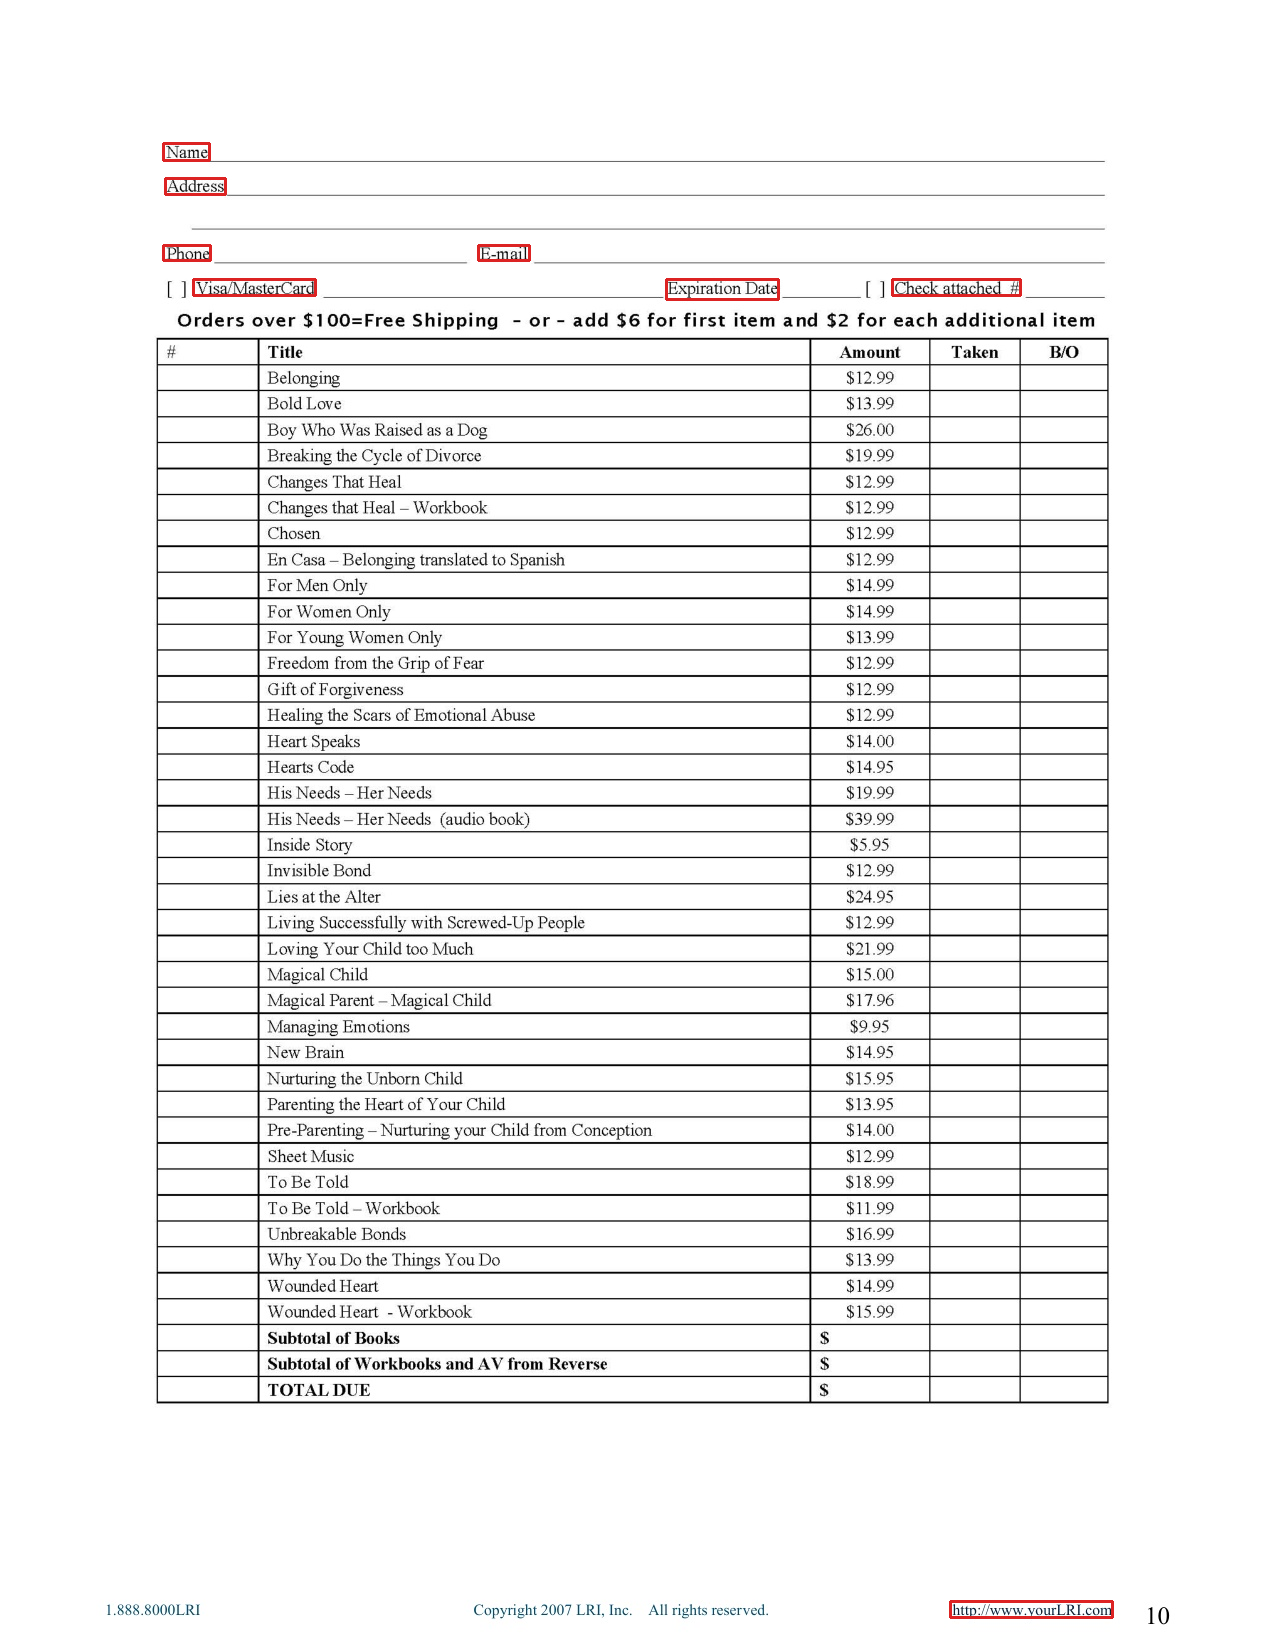
\includegraphics[height=0.44\textheight,trim={70bp 0bp 70bp 100bp},clip]{figures/stage2/stage2_cluster_0_example.png}
        \par\smallskip
        \textbf{(a)} Page with annotations across a broad area
    \end{minipage}\hfill
    \begin{minipage}[t]{0.52\textwidth}
        \centering
        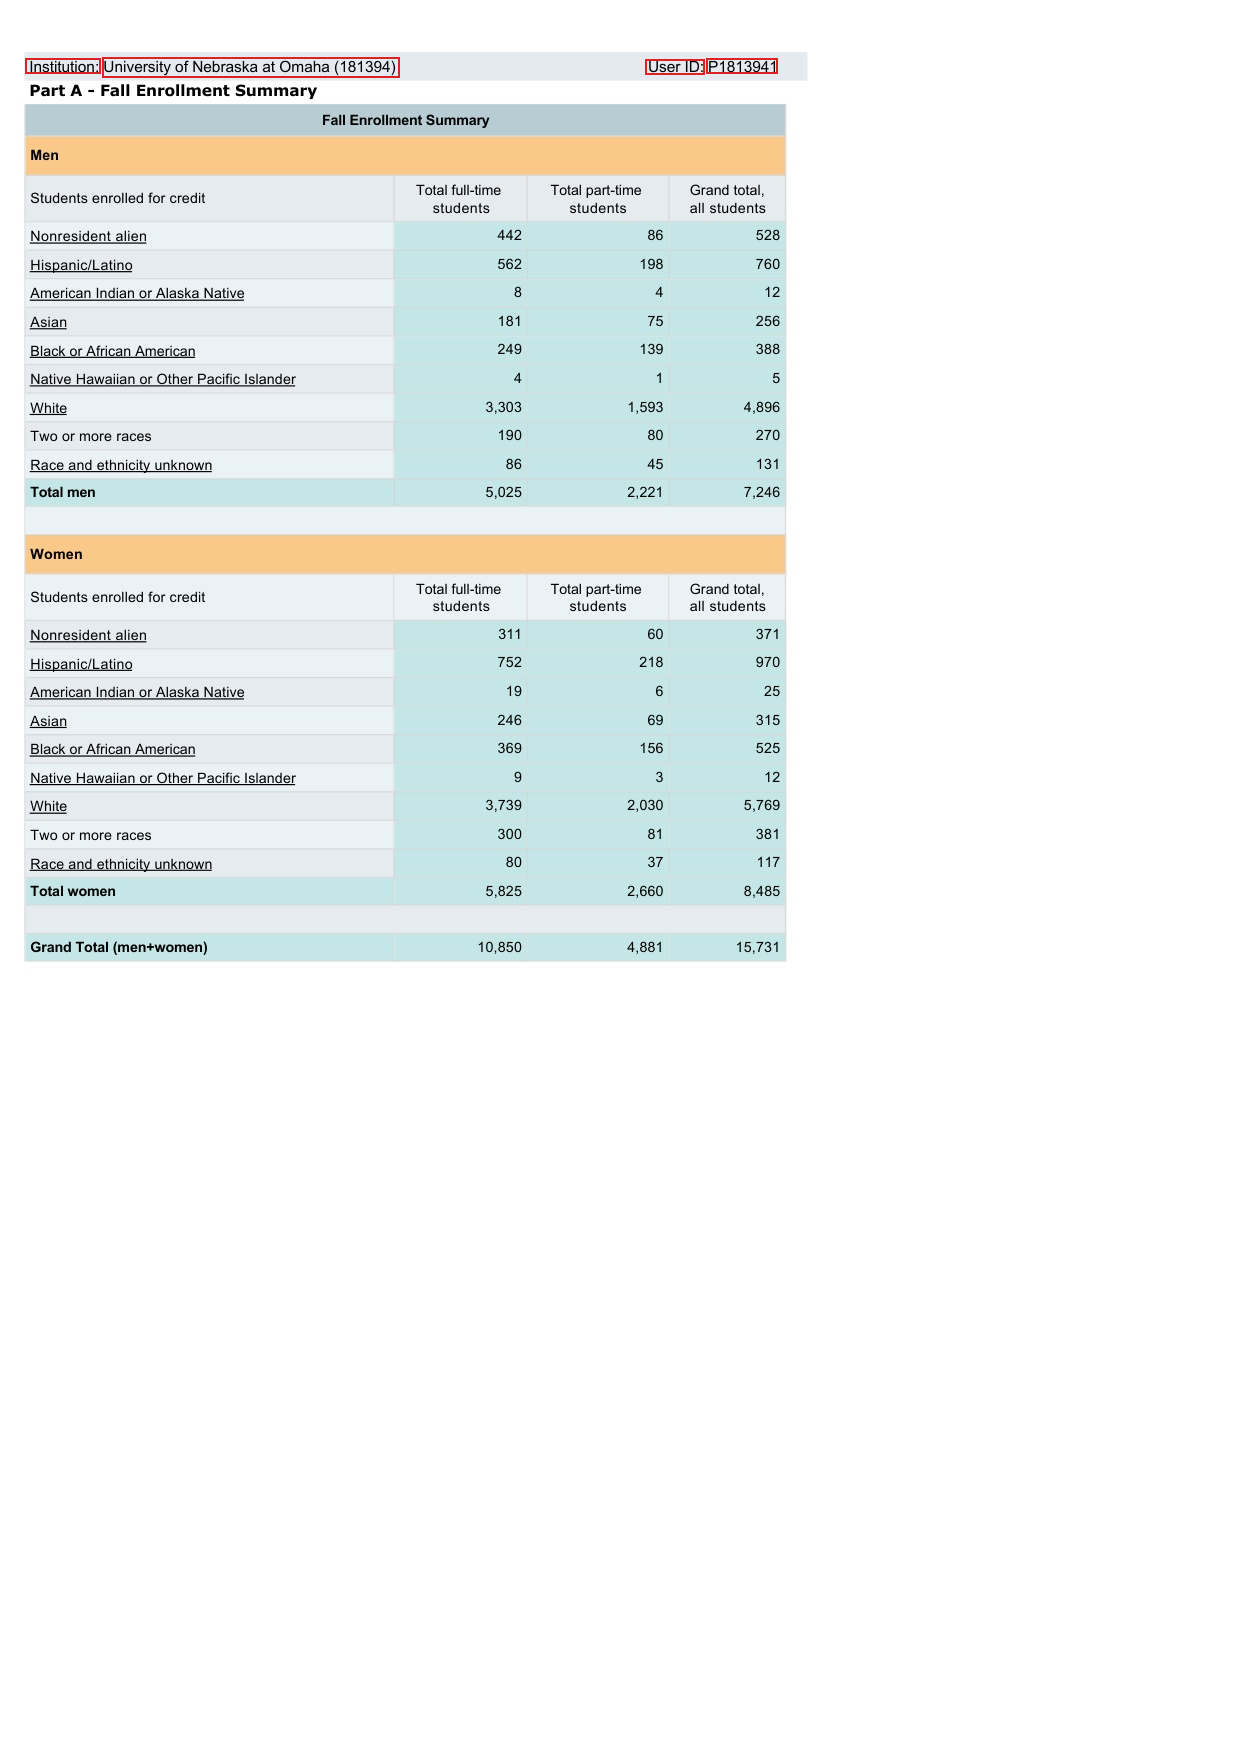
\includegraphics[height=0.44\textheight,trim={0bp 740bp 380bp 20bp},clip]{figures/stage2/stage2_cluster_1_example.png}
        \par\smallskip
        \textbf{(b)} Page with annotations in a more compact area
    \end{minipage}
    \caption{Two illustrative KVP10k test pages with polygon annotation
    overlays. Red outlines mark annotated regions. The pages are used later
    to illustrate the fitted annotation-geometry groups.}
    \label{fig:stage2_cluster_examples}
\end{figure}

\section{Page-Level Annotation-Geometry Clustering}
\label{sec:layout_clustering}

The annotation-geometry analysis creates coarse page groups, called geometry
strata, for later descriptive error analysis. Its input is a page-level
summary of the number, size, position, spread, and spacing of human annotation
polygons. Its output is one geometry-cluster assignment for each
coordinate-bearing page. Later chapters use these assignments to examine
whether extraction performance differs across annotation layouts. The cluster
assignments are not model-training targets.

Raw annotation rows are grouped by \texttt{hash\_name}. For each unique
official-training page, the analysis retains the annotator copy with the
largest number of usable polygons. A coordinate-bearing page is a page for
which this selected copy contains at least one usable polygon. Pages with no
usable coordinates in any copy are excluded instead of being represented by
an artificial all-zero feature vector. This process yields 9{,}124
coordinate-bearing pages from the 9{,}656 unique official-training pages;
532 pages have unavailable annotation geometry.

The fitted groups describe annotation geometry only. They do not establish
document genre, the layout of unannotated page content, or OCR-token density.

\subsection{Feature Extraction}
\label{subsec:features}

For each selected page, the analysis extracts the 12 geometric summary
features in Table~\ref{tab:features}. The original extractor emitted 13
columns, but \texttt{density} was identical to \texttt{total\_area}. The
analysis removes this duplicate before standardization so that the same
quantity does not receive twice the weight.

\begin{table}[h]
\centering
\caption{Distinct geometric summary features extracted from each selected page}
\label{tab:features}
\begin{tabular}{@{}ll@{}}
\toprule
\textbf{Feature} & \textbf{Description} \\ \midrule
$n_{\text{boxes}}$ & Number of bounding boxes \\
$A_{\text{total}}$ & Sum of individual bounding-box areas \\
$\mu_A$ & Mean box area \\
$\sigma_A$ & Standard deviation of box area \\
$\mu_w$ & Mean box width \\
$\mu_h$ & Mean box height \\
$\mu_r$ & Mean aspect ratio (width/height) \\
$\mu_x$ & Mean x-position (horizontal center) \\
$\mu_y$ & Mean y-position (vertical center) \\
$s_v$ & Vertical spread (max$_y$ - min$_y$) \\
$s_h$ & Horizontal spread (max$_x$ - min$_x$) \\
$d_{\text{spacing}}$ & Mean pairwise Euclidean distance between box centers \\ \bottomrule
\end{tabular}
\end{table}

Together, the features describe annotation count, box size, box position,
spatial spread, and pairwise spacing. The feature vector contains no page
pixels, document text, or OCR-token-density measure.

\subsection{K-means Clustering}
\label{subsec:kmeans}

Each feature is standardized with the mean and standard deviation estimated
from the 9{,}124 coordinate-bearing training pages. K-means
clustering~\cite{kmeans} is then fitted with seed 42 and 10 initializations.
For the candidate cluster counts $k \in \{2,\dots,10\}$, the silhouette
score is the primary selection
criterion~\cite{rousseeuw1987silhouettes}. The Davies--Bouldin
index~\cite{davies1979cluster}, Calinski--Harabasz
score~\cite{calinski1974dendrite}, and inertia curve provide supporting
diagnostics. Higher silhouette and Calinski--Harabasz values and lower
Davies--Bouldin values indicate stronger separation. The inertia curve is
inspected for diminishing improvement as $k$ increases.

Figure~\ref{fig:stage2_optimal_k} summarizes the cluster-count diagnostics.
The silhouette score reaches its maximum of $0.222$ at $k=2$, and the
Calinski--Harabasz score is also largest at $k=2$. The Davies--Bouldin index
is lower for several larger values of $k$ and reaches its minimum at $k=10$.
Together, these diagnostics provide only limited evidence for a clean
two-group partition. We retain $k=2$ as the simplest solution selected by the
primary criterion and use the two groups only as exploratory geometry strata.

\begin{figure}[H]
    \centering
    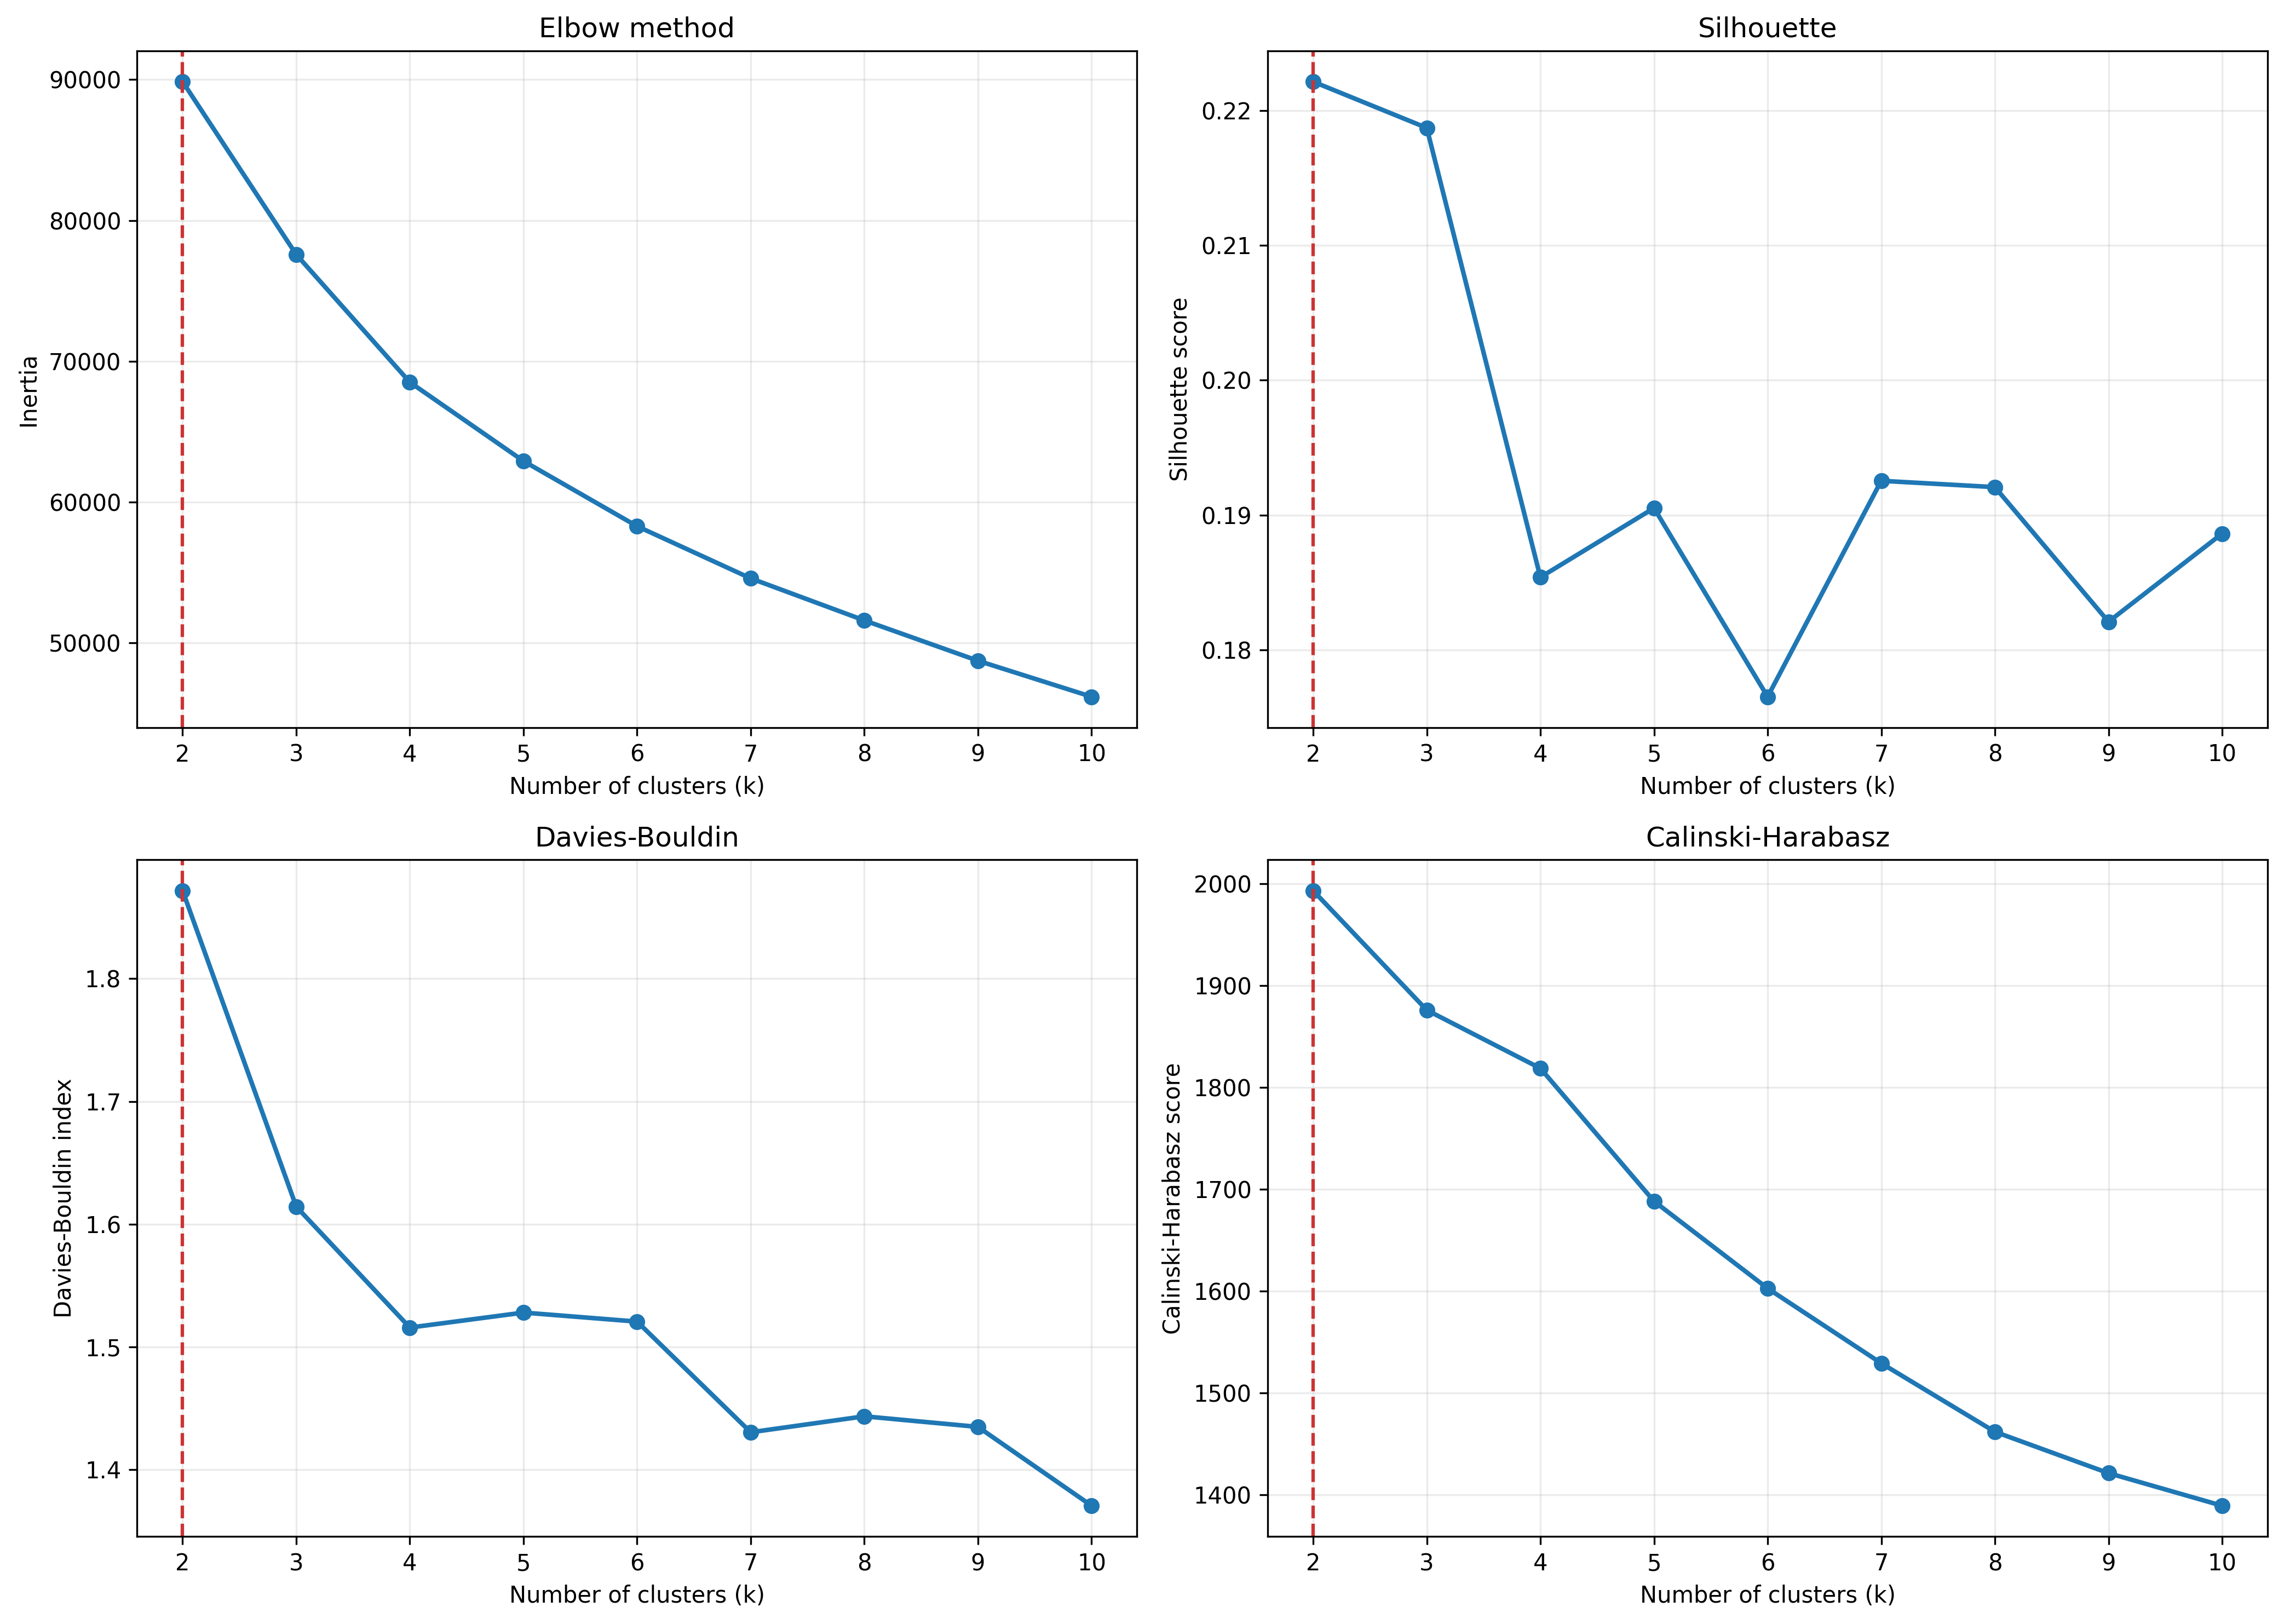
\includegraphics[width=0.75\textwidth]{figures/stage2/optimal_k_analysis.png}
    \caption{Cluster-count diagnostics for the annotation-geometry analysis:
    silhouette score, Davies--Bouldin index, Calinski--Harabasz score, and
    inertia.}
    \label{fig:stage2_optimal_k}
\end{figure}

Table~\ref{tab:clusters} summarises the resulting two-cluster composition.

\begin{table}[H]
\centering
\caption{Page-level geometry-cluster distribution for $k=2$}
\label{tab:clusters}
\begin{tabular}{@{}lrrr@{}}
\toprule
\textbf{Cluster} & \textbf{Pages} & \textbf{\%} & \textbf{Characteristics} \\ \midrule
0 & 5{,}617 & 61.6\% & Higher box count and broader spatial spread \\
1 & 3{,}507 & 38.4\% & Lower box count, larger boxes, and more compact spread \\ \bottomrule
\end{tabular}
\end{table}

Cluster~0 contains 61.6\% of the coordinate-bearing training pages, while
Cluster~1 contains 38.4\%. These proportions describe the geometry-analysis
population only; they are not the proportions of the prepared model-training
or test subsets.

\subsection{Projection and Cluster Interpretation}
\label{subsec:pca}

\Gls{pca}~\cite{pca} projects the standardized 12-dimensional feature
vectors onto two linear components. The first principal component (PC1)
explains 30.1\% of the variance, and the second principal component (PC2)
explains 22.7\%; together they explain 52.8\%.
Figure~\ref{fig:stage2_pca} shows substantial overlap between the groups,
consistent with the modest silhouette score.

\begin{figure}[H]
    \centering
    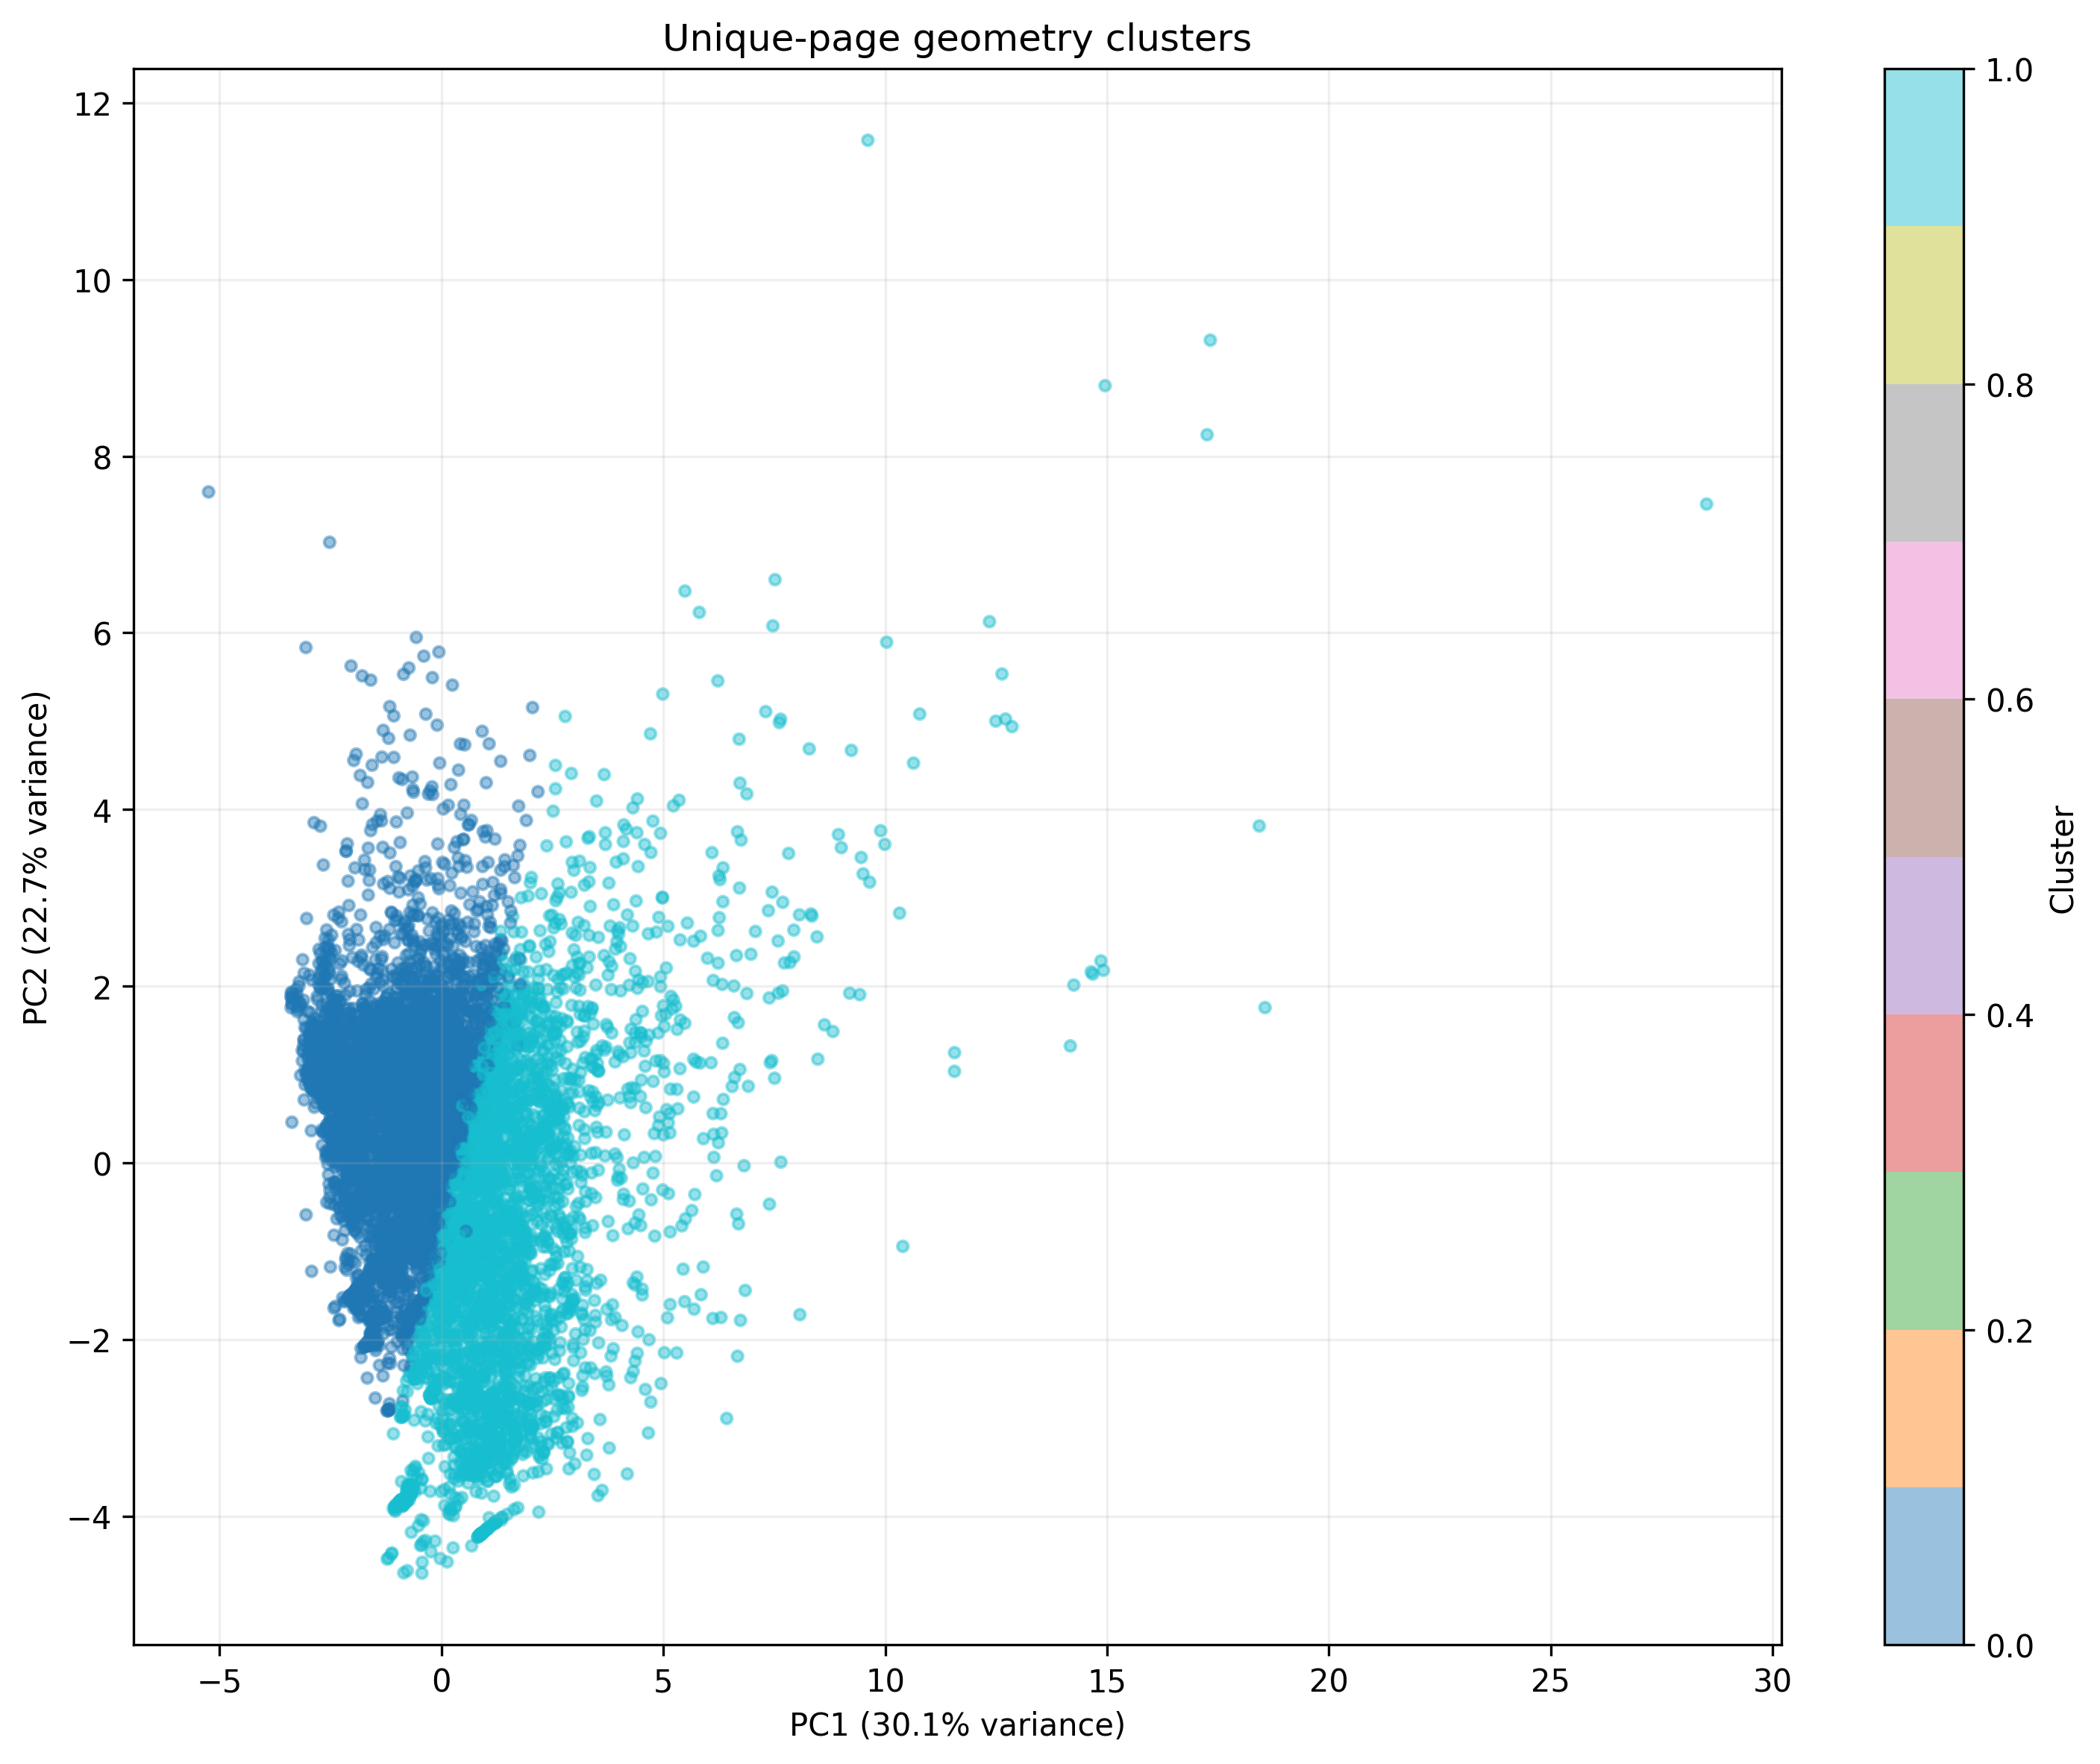
\includegraphics[width=0.80\textwidth]{figures/stage2/pca_clusters.png}
    \caption{PCA visualization of the $k=2$ unique-page geometry clusters.}
    \label{fig:stage2_pca}
\end{figure}

The pages in Figure~\ref{fig:stage2_cluster_examples} illustrate the fitted
groups. Panel~(a) is assigned to Cluster~0, and Panel~(b) is assigned to
Cluster~1. The examples aid interpretation, but they do not establish that
every page in a cluster has the same visual structure.

As a qualitative check, \gls{tsne}~\cite{tsne} provides a nonlinear
two-dimensional projection of a fixed random sample of 3{,}000
coordinate-bearing official-training pages
(Figure~\ref{fig:stage2_tsne}). It uses the same standardized features as
K-means. This visualization is descriptive only and is not used to select
$k$.

\begin{figure}[H]
    \centering
    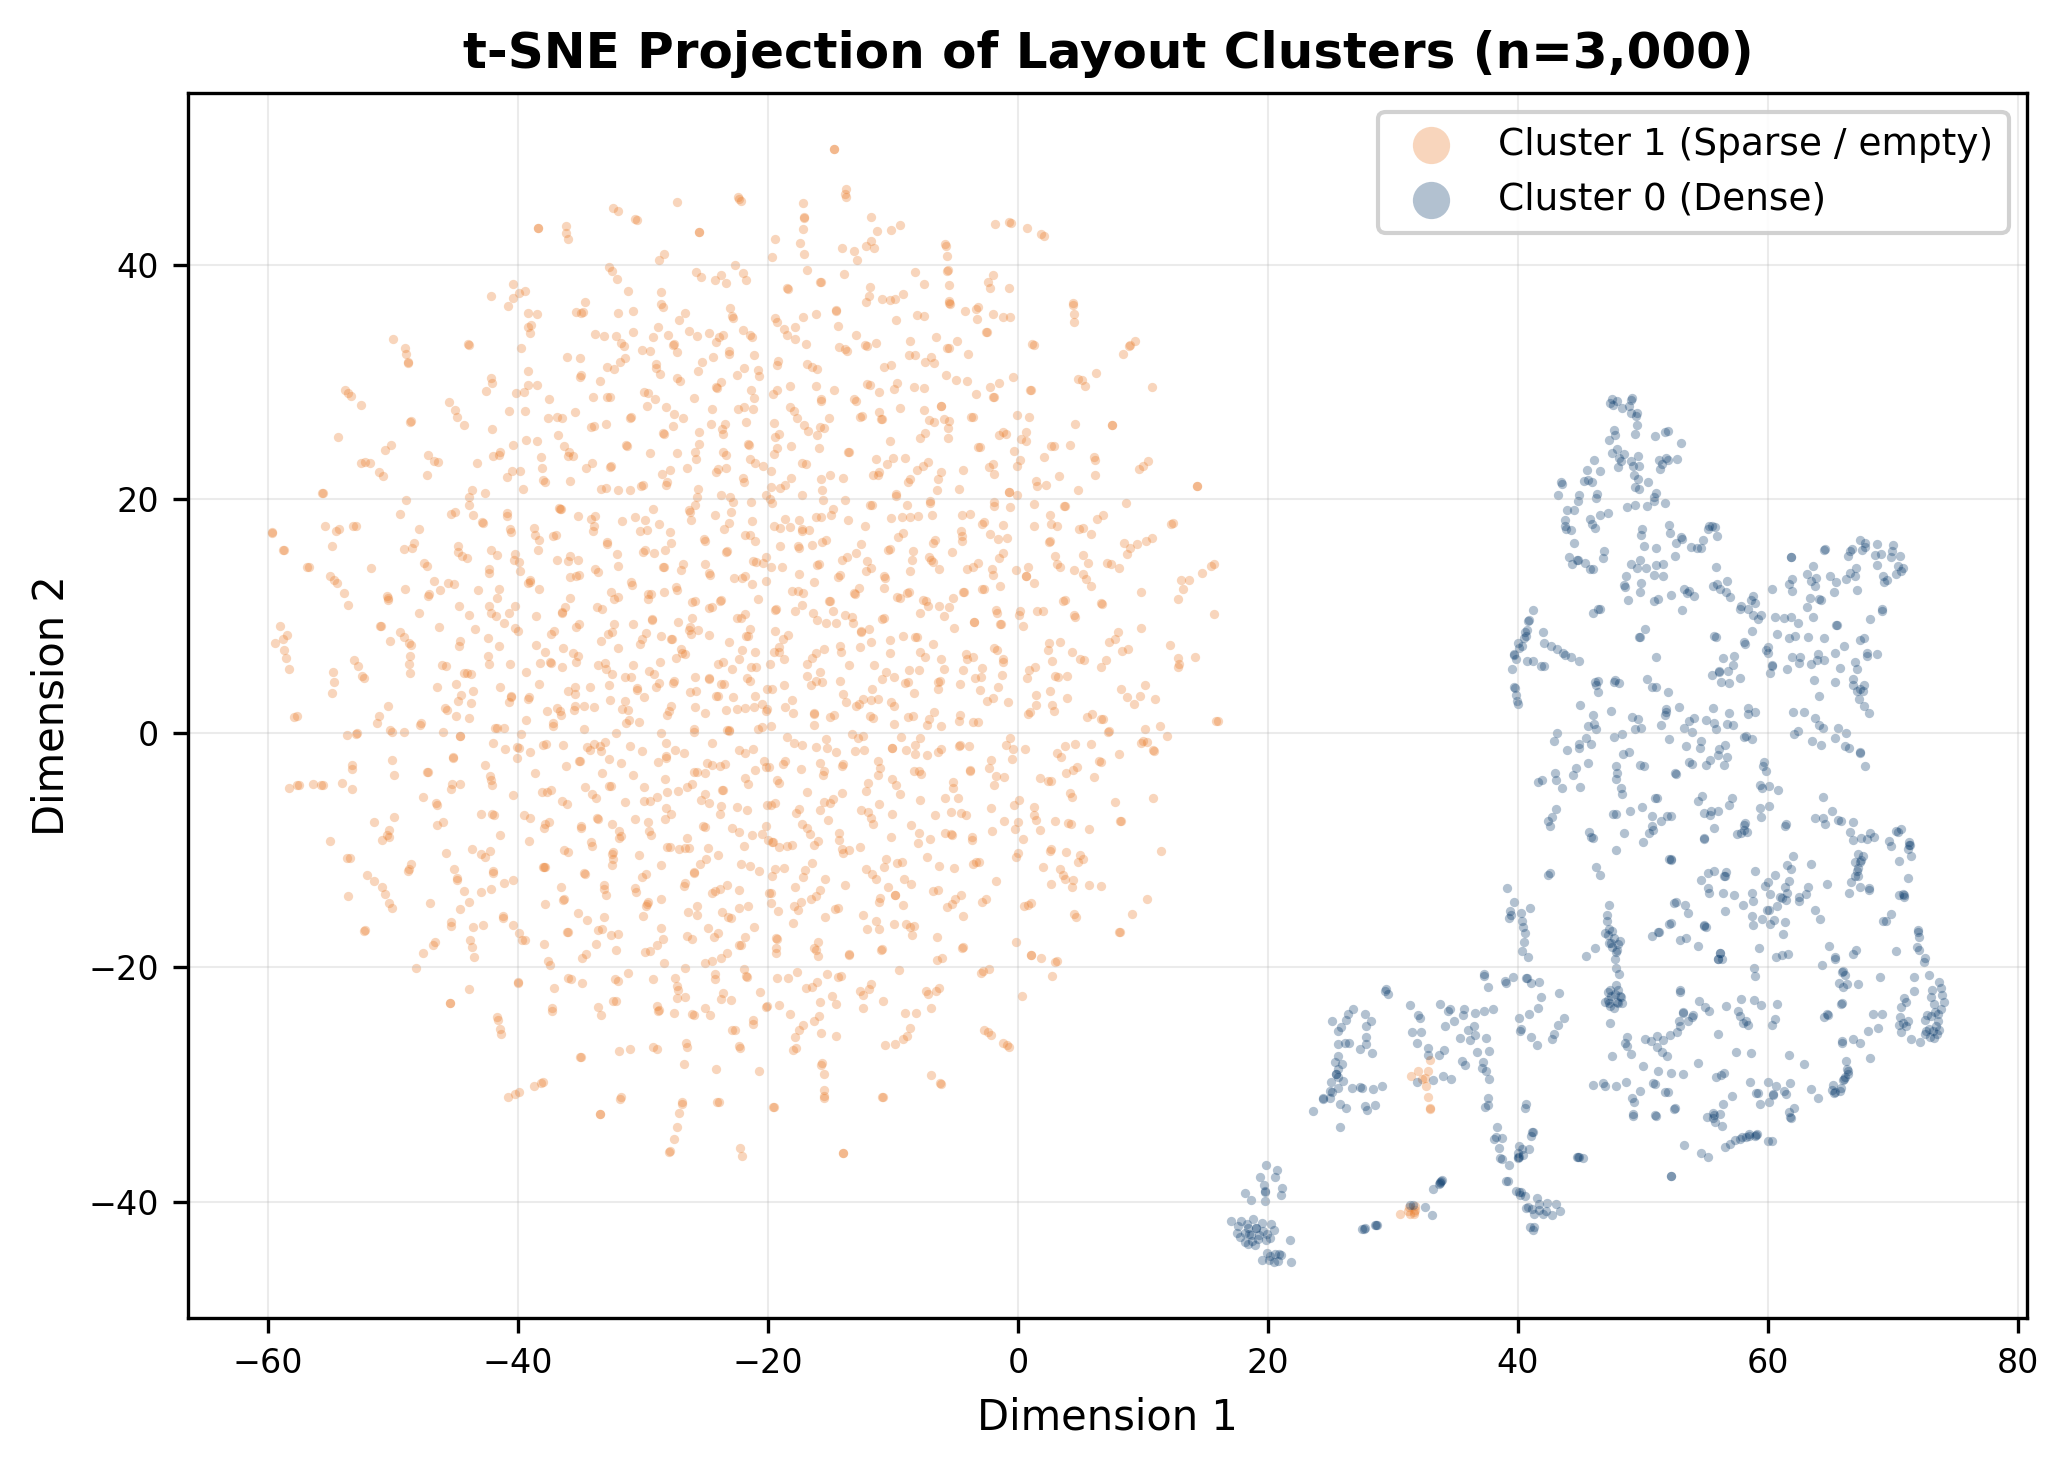
\includegraphics[width=0.72\textwidth]{figures/stage2/tsne_clusters.png}
    \caption{Exploratory t-SNE projection of 3{,}000 unique coordinate-bearing training pages.}
    \label{fig:stage2_tsne}
\end{figure}

To interpret the clusters, Figure~\ref{fig:stage2_feature_distributions} and Table~\ref{tab:stage2_cluster_stats} summarize how key geometry statistics differ across clusters.

\begin{figure}[htbp]
    \centering
    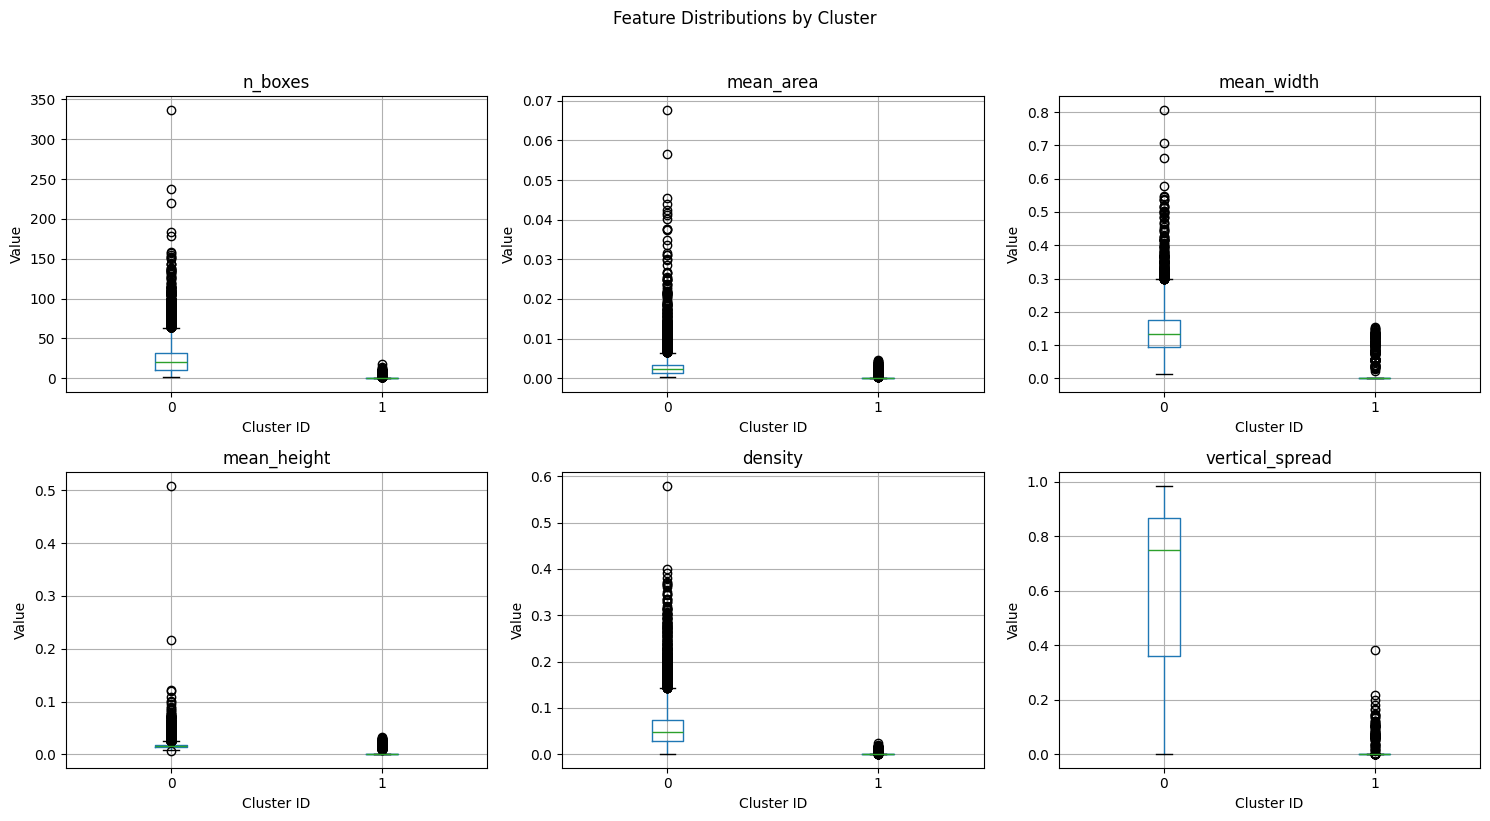
\includegraphics[width=0.90\textwidth]{figures/stage2/feature_distributions.png}
    \caption{Selected geometry-feature distributions for the unique-page clusters.}
    \label{fig:stage2_feature_distributions}
\end{figure}

\begin{table}[H]
    \centering
    \small
    \caption{Summary statistics of selected geometry features per cluster (mean\,$\pm$\,std).}
    \label{tab:stage2_cluster_stats}
    \begin{tabular}{@{}lrrr@{}}
        \toprule
        \textbf{Cluster}
            & \shortstack{\textbf{$n_{\text{boxes}}$}\\\textbf{mean $\pm$ std}}
            & \shortstack{\textbf{Vertical spread}\\\textbf{mean $\pm$ std}}
            & \shortstack{\textbf{Horizontal spread}\\\textbf{mean $\pm$ std}} \\
        \midrule
        0 & $31.659 \pm 22.460$ & $0.714 \pm 0.261$ & $0.739 \pm 0.122$ \\
        1 & $14.206 \pm 10.016$ & $0.421 \pm 0.289$ & $0.372 \pm 0.202$ \\
        \bottomrule
    \end{tabular}
\end{table}

Cluster~0 contains more boxes distributed across a broader portion of the page. Cluster~1 contains fewer boxes with larger mean dimensions and more compact horizontal and vertical spread. These descriptions concern annotation polygons only: they do not establish OCR-token density, document genre, or visual appearance outside the annotated regions.

\subsection{Application to Test Pages and Later Evaluation}
\label{subsec:cluster_use}

The scaler and K-means model are fitted only on the 9{,}124
coordinate-bearing official-training pages. Official-test rows are grouped by
\texttt{hash\_name} and reduced with the same annotator-copy selection rule.
The frozen model assigns 588 of the 1{,}051 unique official-test pages to
Cluster~0 and 396 to Cluster~1. The remaining 67 pages have no usable
annotation geometry and receive the label \emph{geometry unavailable}; they
are not represented by an artificial zero vector.

Within the prepared 581-page evaluation subset, the corresponding counts are
319, 213, and 49. Per-cluster results in later chapters are recomputed from
saved predictions and ground truth; the overall benchmark scores remain
unchanged (Section~\ref{sec:stage3-per-cluster}). An implementation excerpt
for applying the frozen geometry-clustering model is provided in
Appendix~\ref{app:cluster-assignment}.

\section{Key--Value Link Analysis}
\label{sec:kv_analysis}

The spatial-link audit characterizes the center distances of linked key and
value regions. Its purpose is to assess whether spatial proximity is a
plausible input signal for the relation linker; it does not test model
performance.

\subsection{Spatial Proximity}

For each annotation whose linking value resolves to another
coordinate-bearing annotation, the analysis computes the page-normalized
Euclidean distance between the centers of the key and value boxes:

\begin{equation}
d_{kv} = \sqrt{(x_v - x_k)^2 + (y_v - y_k)^2}
\end{equation}

where $(x_k, y_k)$ and $(x_v, y_v)$ are the normalized center coordinates of the key and value boxes.

The audit uses a convenience subset consisting of the first 200
official-training annotation rows with non-empty annotation lists. These rows
represent 70 unique page hashes, and 69 rows contain usable coordinate
information. Across 3{,}595 annotations, 755 contain a non-empty linking
value. The saved audit output also records 755 resolved coordinate-bearing
pair-distance instances. The mean center distance is
$\mu_d = 0.120$, the median is $\tilde{d} = 0.095$, and the 90th percentile
is $d_{90} = 0.239$, all in normalized page-coordinate units.

The observed distances motivate the use of spatial information as a linker
input. They do not measure the effect of spatial features on model
performance. The subset is not a random unique-page sample and contains
several annotator copies for some pages. The values are therefore exploratory
and are not dataset-wide estimates.

\section{Annotation Statistics}
\label{sec:annotation_stats}

Table~\ref{tab:ann_stats} summarizes the units and composition of the
exploratory raw-row subset.

\begin{table}[h]
\centering
\caption{Composition of the exploratory 200-row official-training subset}
\label{tab:ann_stats}
\begin{tabular}{@{}lr@{}}
\toprule
\textbf{Metric} & \textbf{Value} \\ \midrule
Total annotation rows & 200 \\
Unique page hashes & 70 \\
Coordinate-bearing rows & 69 \\
Total annotations & 3{,}595 \\
Mean annotations per row & 17.98 \\
Annotations with non-empty linking values & 755 \\
Share of annotations with linking values & 21.0\% \\ \bottomrule
\end{tabular}
\end{table}

The 755 annotations with linking values constitute 21.0\% of the 3{,}595
annotations in this subset. Because the 200 rows represent only 70 unique
page hashes and were selected by row order, this percentage is not a
dataset-wide prevalence estimate.

\section{Summary}
\label{sec:dataset_summary}

The analysis produces two weakly separated annotation-geometry strata.
Cluster~0 contains pages with more annotation boxes and broader spatial
spread, while Cluster~1 contains pages with fewer boxes and more compact
spread. The strata support descriptive performance analysis only and do not
represent verified document genres or OCR-token-density classes.

In the limited 200-row spatial audit, recovered linked-pair instances have
relatively small normalized center distances. This result motivates the use
of spatial information in the linker, but it does not measure the contribution
of that information to extraction performance.
